%%
%% This is file `sample-sigconf.tex',
%% generated with the docstrip utility.
%%
%% The original source files were:
%%
%% samples.dtx  (with options: `sigconf')
%% 
%% IMPORTANT NOTICE:
%% 
%% For the copyright see the source file.
%% 
%% Any modified versions of this file must be renamed
%% with new filenames distinct from sample-sigconf.tex.
%% 
%% For distribution of the original source see the terms
%% for copying and modification in the file samples.dtx.
%% 
%% This generated file may be distributed as long as the
%% original source files, as listed above, are part of the
%% same distribution. (The sources need not necessarily be
%% in the same archive or directory.)
%%
%%
%% Commands for TeXCount
%TC:macro \cite [option:text,text]
%TC:macro \citep [option:text,text]
%TC:macro \citet [option:text,text]
%TC:envir table 0 1
%TC:envir table* 0 1
%TC:envir tabular [ignore] word
%TC:envir displaymath 0 word
%TC:envir math 0 word
%TC:envir comment 0 0
%%
%%
%% The first command in your LaTeX source must be the \documentclass command.
\documentclass[sigconf]{acmart}

\usepackage{pgfplotstable}

\setlength {\marginparwidth }{2cm}
\usepackage[colorinlistoftodos]{todonotes}
\usepackage{tabularx}
\usepackage{pgfplots}
\usepackage{enumitem}
\pgfplotsset{compat=1.17}
\usetikzlibrary{calc}

%%
%% \BibTeX command to typeset BibTeX logo in the docs
\AtBeginDocument{%
  \providecommand\BibTeX{{%
    \normalfont B\kern-0.5em{\scshape i\kern-0.25em b}\kern-0.8em\TeX}}}

%% Rights management information.  This information is sent to you
%% when you complete the rights form.  These commands have SAMPLE
%% values in them; it is your responsibility as an author to replace
%% the commands and values with those provided to you when you
%% complete the rights form.
\setcopyright{acmcopyright}
\copyrightyear{2021}
\acmYear{2021}
\acmDOI{}

%% These commands are for a PROCEEDINGS abstract or paper.
\acmConference[K-Cap '21]{K-Cap '21: The Eleventh International Conference on Knowledge Capture}{December 02--03, 2021}{Virtual Conference}


%%
%% Submission ID.
%% Use this when submitting an article to a sponsored event. You'll
%% receive a unique submission ID from the organizers
%% of the event, and this ID should be used as the parameter to this command.
%%\acmSubmissionID{123-A56-BU3}

%%
%% The majority of ACM publications use numbered citations and
%% references.  The command \citestyle{authoryear} switches to the
%% "author year" style.
%%
%% If you are preparing content for an event
%% sponsored by ACM SIGGRAPH, you must use the "author year" style of
%% citations and references.
%% Uncommenting
%% the next command will enable that style.
%%\citestyle{acmauthoryear}

%%
%% end of the preamble, start of the body of the document source.
\begin{document}

%%
%% The "title" command has an optional parameter,
%% allowing the author to define a "short title" to be used in page headers.
\title{OntoFlow : Easy Ontology Development Workflows for working with Non-technical Domain Experts}

%%
%% The "author" command and its associated commands are used to define
%% the authors and their affiliations.
%% Of note is the shared affiliation of the first two authors, and the
%% "authornote" and "authornotemark" commands
%% used to denote shared contribution to the research.
\author{Gordian Dziwis}
\authornote{}
\email{dziwis@infai.org}
\author{Lisa Wenige}
\authornotemark[1]
\email{wenige@infai.org}
\author{Lars-Peter Meyer}
\authornotemark[1]
\email{lpmeyer@infai.org}
\affiliation{%
  \institution{Institute for Applied Informatics}
  \streetaddress{Goerdelerring 9}
  \city{Leipzig}
  \state{Saxony}
  \country{Germany}
  \postcode{04177}
}

%%
%% By default, the full list of authors will be used in the page
%% headers. Often, this list is too long, and will overlap
%% other information printed in the page headers. This command allows
%% the author to define a more concise list
%% of authors' names for this purpose.
\renewcommand{\shortauthors}{Dziwis and Wenige et al.}

%%
%% The abstract is a short summary of the work to be presented in the
%% article.
\begin{abstract}
  For many years, the development of widely applicable and high quality ontologies has been an ongoing research topic. Among the many challenges, the lack of integrated development environments for non-technical domain experts has been one of the most pressing research challenges. But while the participation of domain experts is vital for the applicability of ontologies, there are hardly any software tools available that facilitate their active engagement. We present a solution that addresses this research gap by automating the ontology development process with the help of a workflow engine. We define a pipeline that facilitates ontology implementation, serialization, documentation and testing within the scope of a seamless automatic routine than can be easily triggered by an ontology laymen with basic knowledge of bash usage. Thus, the processing pipeline takes care of most of the operations that usually have to be taken care of by an ontology or software engineer. We demonstrate the applicability of our approach for a wide range of ontologies and provide additional results on the quality level of ontologies throughout the Semantic Web landscape.
\end{abstract}

%%
%% The code below is generated by the tool at http://dl.acm.org/ccs.cfm.
%% Please copy and paste the code instead of the example below.
%%
%\begin{CCSXML}
%  <ccs2012>
%  <concept>
%  <concept_id>10010520.10010553.10010562</concept_id>
%  <concept_desc>Computer systems organization~Embedded systems</concept_desc>
%  <concept_significance>500</concept_significance>
%  </concept>
%  <concept>
%  <concept_id>10010520.10010575.10010755</concept_id>
%  <concept_desc>Computer systems organization~Redundancy</concept_desc>
%  <concept_significance>300</concept_significance>
%  </concept>
%  <concept>
%  <concept_id>10010520.10010553.10010554</concept_id>
%  <concept_desc>Computer systems organization~Robotics</concept_desc>
%  <concept_significance>100</concept_significance>
%  </concept>
%  <concept>
%  <concept_id>10003033.10003083.10003095</concept_id>
%  <concept_desc>Networks~Network reliability</concept_desc>
%  <concept_significance>100</concept_significance>
%  </concept>
%  </ccs2012>
%\end{CCSXML}

%\ccsdesc[500]{Computer systems organization~Embedded systems}
%\ccsdesc[300]{Computer systems organization~Redundancy}
%\ccsdesc{Computer systems organization~Robotics}
%\ccsdesc[100]{Networks~Network reliability}

%%
%% Keywords. The author(s) should pick words that accurately describe
%% the work being presented. Separate the keywords with commas.
\keywords{Ontology, Workflow, Integrated Development Environment, Quality Assurance}

%%
%% This command processes the author and affiliation and title
%% information and builds the first part of the formatted document.
\maketitle

\section{Introduction}
With the proliferation of knowledge graphs, ontology development has become a central part of data integration activities. Due to the increasing efforts around FAIR data and research data infrastructures worldwide \cite{fair}, collaborative and decentralized processes around ontology development are on the rise. However, available software tools fall short of the multi-layered requirements of ontology development which comprise labour-intensive tasks such as ontology modeling, serialization, validation and documentation. Moreover, these tasks often have to be carried out collaboratively and in a decentralized manner, as several (often geographically dispersed) groups of people are involved in the ontology development process thus making it a multi-stakeholder endeavor \cite{sure}. In addition to that, many of the tools available are difficult to handle for domain experts without IT or Semantic Web background \cite{tudorache}. While these experts usually have an extraordinarily high level of expertise in their field (e.g., in life sciences, physics or cultural heritage) they might not be as familiar with the methods and tools commonly applied in software and knowledge graph engineering. This situation is exacerbated by the fact that there exists no standard tool stack for ontology development in the Semantic Web community so far. Although some tools, such as Protégé \cite{protege}, are considerably widespread, they only cover partial aspects of the engineering process such as ontology modeling or editing and cannot be used in the sense of a fully-fledged integrated development environment (IDE). On top of that, many software tools for RDF file processing can either only be used as a command-line utility and/or provide limited usability in terms of a graphical user interface (GUI). However, the possibilities of containerizing tools and automating workflows by applying principles of continuous integration (CI) practices from software engineering provide novel opportunities for supporting ontology development \cite{fowler}. They can also help to ease participation of domain experts in these processes.\\
With Ontoflow we propose a solution that bundles several necessary operations of ontology engineering in a single automated workflow by adopting best practices from continuous integration and deployment (CI/CD) pipelines \cite{humble}. Thus, we are able to integrate ontology modeling, serialization, testing and documentation in a unified process which makes time-consuming, repetitive and error-prone manual work mostly superfluous. 
The paper is structured as follows: Section \ref{sec:related} provides an overview of current practices of workflow automation for data collections and highlights existing gaps in software-based support for ontology development processes. Section \ref{sec:ontoflow} introduces requirements, architecture and implementation-specific details of the OntoFlow approach. Section \ref{sec:eval} presents results of the evaluation of the OntoFlow approach, while the final section () summarizes the most important findings and propososes directions for future work \ref{sec:final}.

\section{Related Work}
\label{sec:related}
Continuous development and integration strategies have become an indispensable part of modern software engineering.
They largely consist of clean up operations, compilation of executables, application of automated tests, and the deployment of the finished application, including generation of appropriate documentation if necessary. Part of these processes is the continuous checking of any updates/ new versions as well as the triggering of troubleshooting activities if problems occur \cite{fowler}.
This ensures that software solutions are always up-to-date, that applications meet predefined quality standards and rely on stable software artifacts.\\
Likewise, in the wake of ever-growing data volumes and increased relevance of data-driven applications, effective mechanisms to control the quality-assured publication of data products have become important requirements for IT operations. Processes that follow Continuous Integration (CI) principles are equally applicable when the production of data artifacts in collaborative environments should be made more efficient. The knowledge graph community has been one of the first to adopt DevOps best practices for datasets since it heavily relies on high quality data schemas and reproducible workflows for data conversion, integration and fusion. In this line of research, several authors have proposed automated data pipelines that not only take care of data transformation but also apply quality assurance operations and automatic procedures for data publication and effective description of data artifacts
\cite{cirulli, klimek, kucera, meissner, rojas, roman, stadler, dataid}. Typically, CI mechanisms for data collections involve operations such as crawling, linking, or data transformation. These processes are usually executed automatically and, aside from the effort of creating specifications for data conversion, are little interrupted by user interactions and manual intervention. If people work with appropriate software tools in this context, they are mostly data scientists or software engineers.\\
This modus operandi differs from the determining factors in ontology development processes. The creation of an ontology usually involves several experts with diverse backgrounds and different levels of technical expertise. Therefore, an effective ontology development environment/pipeline has to foster collaboration as well as provide a graphical editor in order to effectively support development processes. By this means, even domain experts with little IT expertise can actively take part in the creation of ontologies.\\
Ontology editors such as Protégé \cite{protege}, Vocol \cite{halilaj} or WebVOWL \cite{lohmann} are already established software tools for ontology development and visualisation. Meanwhile, other applications in this area focus more on aspects of collaborative and version-based storage of ontologies so that changes can be managed decentrally and tracked over time. Software tools, such as Ontoology \cite{alobaid} or the QuitStore \cite{arndt} provide solutions for these kinds of requirements.\\
Other tools, such as Oops! focus more on the aspect of quality assurance \cite{poveda} while general purpose RDF data testing suites, such as RDFUnit \cite{rdfunit} or pySHACL\footnote{\url{https://github.com/RDFLib/pySHACL}} can be equally applied for ontology testing. Just as important as quality assurance of ontologies is documentation prepared for end users in a form understandable by users. Software applications that automatically generate ontology documentations are WIDOCO \cite{widoco}, LODE \cite{lode} or pyLODE\footnote{\url{https://github.com/RDFLib/pyLODE}}. They create a HTML representation from ontologies in standard RDF serialization formats.\\
The ROBOT framework \cite{jackson} offers many operations needed for ontology manipulation in the development process, but lacks workflow capabilities according to \cite{jackson}. The ROBOT documentation refers e.g. to the rather technical oriented make\footnote{\url{https://www.gnu.org/software/make/}} tool for more complex needs.\\
So although software applications are already available that support collaborative ontology development processes and also automate them in parts, there is a lack of approaches since \cite{mungall} as to how these processes can be linked in the sense of a CI pipeline while at the same time ensuring that laymen can actively participate in development through making changes and triggering ontology updates.
\todo{https://www.nature.com/articles/s41587-020-0439-x}

\section{Ontology Development Workflow}
\label{sec:ontoflow}
\subsection{Requirements}

% Please add the following required packages to your document preamble:
% \usepackage{booktabs}
% \usepackage{multirow}
\begin{table*}[htb]
\begin{tabular}{@{}lll@{}}
\toprule
Main Requirement &
  Sub-Requirement &
  Explanation \\ \midrule
\textbf{RQ1 ODP Automation} &
  RQ1.1 Ontology serialization &
  \begin{tabular}[l]{@{}l@{}}Ontology artifacts can be automatically \\ serialized in common RDF formats \\ (e.g., RDF/XML, Turtle or NTRIPLES\end{tabular} \\\\
 & 
  RQ1.2 Ontology Validation &
  \begin{tabular}[l]{@{}l@{}}Automatic testing of ontology artifacts\\ is integrated\end{tabular} \\\\
 &
  RQ1.3 Ontology Postprocessing &
  \begin{tabular}[l]{@{}l@{}}Intgrating automatic postprocessing \\ operations, such as updating meta-information, \\ version control or diff detection\end{tabular} \\\\
 &
  \begin{tabular}[l]{@{}l@{}}RQ1.4 Ontology Publication and \\ Documentation\end{tabular} &
  \begin{tabular}[l]{@{}l@{}}Automatic deployment of ontology artifacts \\ (serialization and HTML documentation) to a server\end{tabular} \\\\
\textbf{RQ2 High (Re-)Usability} &
  RQ2.1 GUI support &
  \begin{tabular}[l]{@{}l@{}}Support of ontology modelling through \\ a GUI\end{tabular} \\\\
 &
  \begin{tabular}[c]{@{}l@{}}RQ2.2 Easy execution ontology workflows\end{tabular} &
  \begin{tabular}[c]{@{}l@{}}Domain experts (with little to no IT background)\\ should be able to trigger ontology workflows\end{tabular} \\\\
 & 
 \begin{tabular}[c]{@{}l@{}}RQ2.3 Fast execution of ontology workflows\end{tabular} &
  \begin{tabular}[c]{@{}l@{}}It should be possible to quickly generate an ontology, \\ validate it and create its documentations\end{tabular} \\\\
   &
  \begin{tabular}[c]{@{}l@{}}RQ2.4 Easy modification of ontology workflows\end{tabular} &
  \begin{tabular}[c]{@{}l@{}}Ontology developers should be able to modify them easily to suit their individual requirements \end{tabular} \\\\
\hline
\end{tabular}
\caption{Requirements for OntoFlow}
\label{tab:req}
\end{table*}

The goal of OntoFlow is the best possible optimization and automation of ontology development processes which typically currently involve a great number of labor-intensive tasks, such as modeling, serialization, updating testing and documentation. Due to the fact that such development processes are carried out by several stakeholders, the workflow environment should foster a collaborative and decentralized way of working.\\
Since the development of ontologies often involves domain experts who have only limited expertise in the field of software and data engineering, OntoFlow should provide a GUI for editing the ontology, while automating the most common tasks (e.g., bash scripting and git interaction) in the background. Due to the limited IT experience of some of the involved stakeholders, it is also vital that workflows can be triggered without in-depth technical understanding of software development or semantic technologies. Reducing the amount of necessary skills for the domain expert is critical, because generally ontology development is a one time job for them. A reusable ontology workflow setup directed at domain experts helps avoiding costs for learning the involved technologies and setting up a development and hosting infrastructure (e.g., running a web server for publishing the ontology and documentation) which - apart from working time - can incur further costs for licences and hardware. Because there is no established methodology for ontology development and it happens in diverse environments, OntoFlow must be flexible and facilitate easy modifications to accommodate for different needs.\\
Table \ref{tab:req} gives an overview of the requirements detailed in the above sections.

\subsection{Workflow Structure}

\begin{figure}[h]
  \centering
  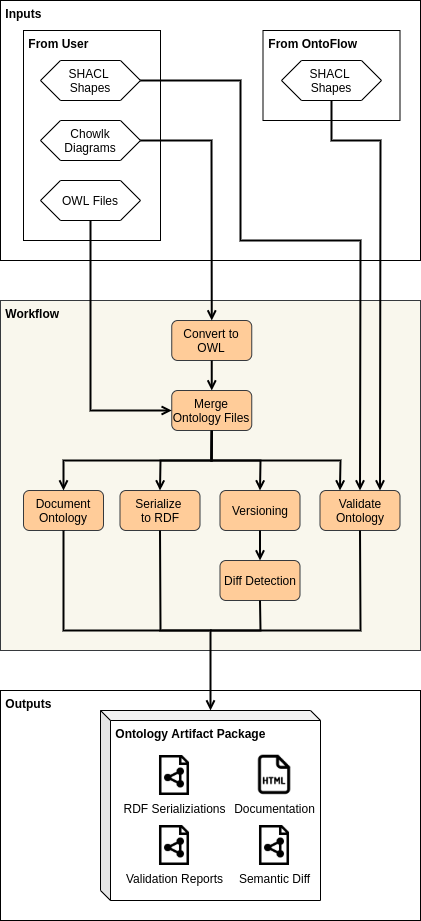
\includegraphics[scale = 0.4]{workflow.png}
  \caption{OntoFlow Workflow}
  \label{fig:workflow}
\end{figure}

Inputs for the workflow are provided by the ontology developer and OntoFlow.
The ontology developer provides ontology diagrams, OWL files and validation shapes.
A ontology diagram is visual representation of an ontology.
The OWL files define ontologies with the Web Ontology Language (OWL) and are serialized as a RDF file.
The ontology is validated against the validation shapes to ensure satisfies a set of conditions.
A set of validation shapes, which test the ontology for formalizable best practice, are supplied by OntoFlow.\footnote{https://gitlab.com/kupferdigital/ontoflow/-/tree/master/shacl}

First process step is the transformation of the ontology diagrams to OWL files and merging those with those OWL files provided by the user.
The resulting ontology is the input for the following parallel processing steps.
A HTML documentation is generated, describing the ontology's metadata, classes and properties.
The ontology is serialized into multiple RDF formats.
In the ontology validation process step, the ontology is validated against the user's and OntoFlow's shapes.
OntoFlow picks up the `owl:priorVersion` property and detects semantic differences to the previous version. This gives an overview which classes changed in the current version compared to the prior version.

The serializations, documentation, validation reports and the semantic differences compose the Ontology Artifact Package.

\subsection{Implementation and Architecture}

\begin{figure}[h]
  \centering
  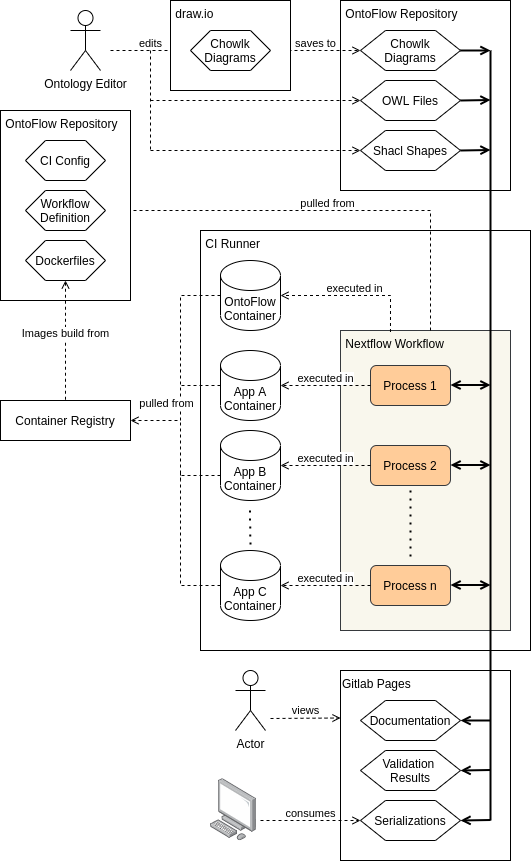
\includegraphics[width=\columnwidth]{architecture.png}
  \caption{OntoFlow Architecture}
  \label{fig:architecture}
\end{figure}

The architectural model for OntoFlow is a pipeline consisting of processes where each process takes inputs, transform the inputs and outputs the results.
Inputs and output from the processes are interconnected.
Each process's transformation is applied to the inputs by application program with a command-line interface.
All applications are containerised and the container images are defined by an definition file.
A workflow engine manages the containers' life cycle and executes the applications and pipes the inputs and outputs between the processes.
The pipeline process steps, with their corresponding commands to execute, their executing containers, inputs and outputs are defined in a workflow definition file.
Each application container is based on a image for which a configuration file exists.
There is a container for OntoFlow itself, which has all the dependencies necessary for running the workflow engine.
The images are hosted in a container registry.
A continuous integration script builds the images and pushes them to the container registry.
Those file are managed inside a version control system.

The diagrams and files defining the ontology are also hosted in a repository.
OntoFlow provides a continuous integration script, which triggers when a change in the ontology repository occurs.
When triggered the OntoFlow container is started with ontology repository mounted.
Inside the container the workflow engine starts the workflow with the files from the ontology repository and OntoFlow's validation shapes as inputs.
Each process step is then executed in its defined application container.
The final outputs are deployed to their target environment.


The pipeline was implemented as a Nextflow workflow and Docker was chosen as the container engine.
For each tool used in a process step a Docker image was created, if not one already existed.
Following is a list of the used tools and their tasks:

\begin{itemize}
  \item Chowlk Converter\footnote{https://github.com/oeg-upm/Chowlk}: Converts ontology diagram to OWL-File.
  \item pySHACL: Validates ontology against SHACL shapes.
  \item Bubastis\footnote{https://github.com/EBISPOT/bubastis}: Creates a semantic diff to an older ontology version./todo{cite https://academic.oup.com/bioinformatics/article/26/8/1112/208992}
  \item Jena Riot\footnote{https://jena.apache.org/documentation/io/}: Serialises and merges RDF-Files.
  \item sparql-integrate\footnote{https://github.com/SmartDataAnalytics/RdfProcessingToolkit}: Extracts and manipulates Data in RDF-Files.
  \item pyLODE: Create ontology documentation in HTML.
\end{itemize}

Chowlk provides a library of owl diagram elements for draw.io, which is an open source diagram software.
OntoFlow can be run on any Linux system with Java and Docker installed.
Which is useful for prototyping and developing OntoFlow, or for getting a quick overview for an ontology by creating its documentation.
To further automation and remove the of setting up infrastructure OntoFlow is integrated into the GitLab ecosystem.
OntoFlow itself and the ontology, which is developed, are hosted on GitLab.
GitLab's container registry hosts the tool images, its continuous integration infrastructure is utilized for running OntoFlow and the Ontology Artifact Package of an ontology is hosted as a GitLab page.
With the ontology files hosted in a GitLab repository, it is possible to edit the ontology collaboratively, because Draw.io can use a GitLab repository as its storage backend.
This also works when multiple persons are editing the same diagram.
This gives collaborative editing without the user being exposed to git.
Chowlk diagrams are Draw.io diagrams of an ontology or parts of an ontology.
They are defined with elements from the Chowlk Ontology Visual Notation library, exported to a XML-File.
A linewise diff comes for free through the usage of a git repository.
For documentation purposes the sematic diff provided by Bubastis gives a more useful overview over the changes between ontology versions.
Bubastis analyzes and reports on the five major types of ontology changes.
Before a diff can be created for an ontology, a serialization and the location of the previous ontology version has to be aquired. To achieve this we build a process step where a SPARQL query is defined which is run against the input RDF file by sparql-integrate and outputs the URI locating the previous ontology version.
\todo{round up and finish}

\section{Evaluation}
\label{sec:eval}
In order to validate our approach, we evaluated to what extent the requirements formulated in Section \ref{sec:ontoflow} are met by OntoFlow. With regard to the functional requirements, corresponding proof of successful functioning is provided through the implementation and successful testing of the execution of the individual components of the OntoFlow workflow against the background of real world use cases. Therefore, OntoFlow was tested in the context of ontology development in materials science with a special focus on copper alloys. Several experts and institutes are currently involved in the development of a copper ontology. The copper ontology should be able to semantically represent the work involved in the development of copper materials, from ore extraction and alloy development to production and recycling of the material. Accordingly, the ontology also consists of several components that can each be modeled with Chowlk, subsequently processed, merged and documented with OntoFlow. The advantage of the approach is that domain experts can work independently as well as collaboratively on the separate ontology components as the corresponding files are stored in a GitLab repository which can be synchronized with draw.io. A beta version of the copper ontology is publicly available and was successfully tested with the OntoFlow.\footnote{\url{https://gitlab.com/kupferdigital/ontology}} 
On top of that, we verified the proper execution of OntoFlow by testing it on a large-scale benchmark dataset of publicly available ontologies to be able to make some valid statements about scalability and applicability of our approach for a wide range of domains. 
We obtained this benchmark dataset from the ontology repository \textit{Linked Open Vocabularies} and downloaded the corresponding ontology files.\footnote{\url{https://lov.linkeddata.es/dataset/lov/sparql}} We decided to use LOV as a reference point for benchmark generation as it is one of the most comprehensive collections of ontologies and vocabularies throughout the Semantic Web \cite{lov}. In total, we extracted 988 files from the LOV registry\footnote{\url{https://gitlab.com/kupferdigital/ontoflow-benchmark/-/tree/main/ontologies}}. From this collection, we determined those files that are lightweight taxonomies and vocabularies (e.g., SKOS thesauri) and removed them from the benchmark as they are not ontologies in a strict sense. In this way, 799 actual ontologies remained. We counted the number of triples of the ontologies and processed each ontology with OntoFlow. We logged the processing time and additional information on whether the workflow completed successfully. From the \todo{count} ontologies \todo{count} were processed successfully.\todo{why did the rest fail}. Hence, it can be concluded that OntoFlow provides a stable environment for the generation, serialization, validation, postprocessing and publication of ontologies. The successful execution of the workflow for such a large number of ontologies demonstrates that OntoFlow is a valuable software tool for automating ontology development processes for a wide range of application domains. The integration of the individual components from the requirements analysis worked largely without errors, so that it can be assumed that the originally identified functionalities for the automation of ontology development could be successfully integrated. The following list summarizes the OntoFlow functionalities with regard to the previously identified requirements an in light of the insights that were gained during the use case and benchmark evaluations. 

\begin{itemize}[leftmargin=*]
\item \textit{RQ1.1 Ontology Serialization:} OntoFlow can output any RDF serialization supported by Apache Riot.
\item \textit{RQ1.2 Ontology Validation:} The ontology is validated against the user provided and OntoFlow's SHACL shapes and the result is added to the output.
\item \textit{RQ1.3 Ontology Postprocessing:} While OntoFlow does pick up a prior version from the ontology and outputs a semantic diff, OntoFlow is not able to add the metadata about versioning during a release automatically.
\item \textit{RQ1.4 Ontology Publication and Documentation:} When set up as a continuous integration Job, OntoFlow completely automates the publishing process. There are two limitations. One is, when published on GitLab pages, the URI has always the schema  

  \mbox{\textit{\url{http(s)://groupname.example.io/projectname}}}. For a own URI a DNS record, which redirects to the GitLab page URI, has to be set up. Second GitLab pages does not support content negotiation\footnote{\url{https://lov.linkeddata.es/dataset/lov/sparql}}. With content negotiation an HTTP client can specify which type (or types) of content it would prefer to receive in response, when it attempts to dereference an URI. For example while a browser accessing the ontology's URI would like to receive the ontology's documentation, a script would prefer to receive a machine readable serialization. 

 \begin{figure}[h]
  \centering
  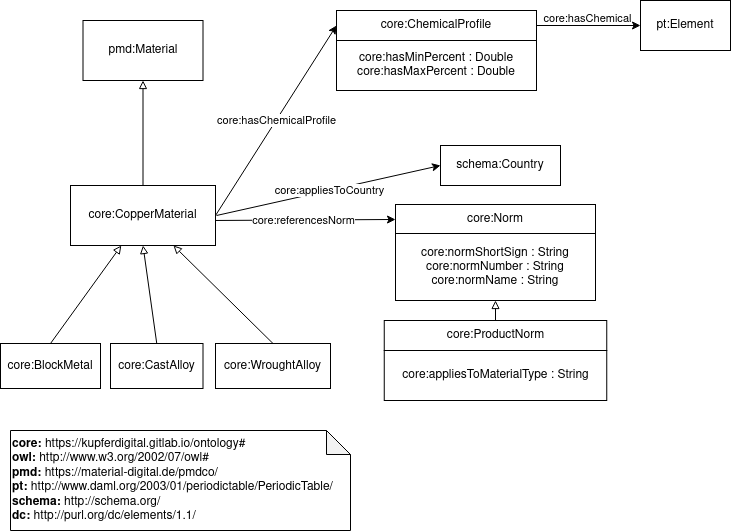
\includegraphics[width=\columnwidth]{copperkey.png}
  \caption{Diagram for the Copperkey Ontology}
  \label{fig:copperkey}
\end{figure}

\item \textit{RQ2.1 GUI support:} The ontology can be build in draw.io with diagram elements from the Chowlk diagram element library, which are extensively documented. \ref{fig:copperkey} shows a diagram which models a part of the copperdigital ontology. Because the Chowlk diagram models OWL and not a general RDF graph, it is not possible to model all aspects of the ontology with a diagram. Metadata like provenance, examples for classes or comments have to be defined in a additional RDF file.
\item \textit{RQ2.2 Easy execution of ontology workflows:} When run as GitLab CI Job the execution happens automatically when draw.io saves the ontology diagram. Setting this automation up is done by copying a CI config file to the ontology repository. Running OntoFlow locally is more involved, because Java, Docker and Nextflow have to be installed and OntoFlow is triggered by a CLI command.
\item \textit{RQ2.3 Fast execution of ontology workflows:} \ref{fig:eval} shows the relationship between the triple count in a ontology and the duration OntoFlow took to process the ontology.
It took OntoFlow at least 17 seconds to process an ontology and the maximum processing duration was 314 seconds for an ontology with 103098 triples.
A linear regression model was a good fit to model the relationship with a coefficient of determination of 0.91.
Workflow execution and time measurements were run on a 4-core laptop with a solid state disk. 
The zoomed graph from \ref{fig:eval}, shows that execution durations are clustered around 25s for most ontologies, but this is for running OntoFlow locally. Execution with the free tier GitLab runner takes about 3-4 minutes. Execution with the GitLab runner takes more time because the free tier Runner only has one core and needs fetch all container images for each run.
\todo{tradeoff containers}
Execution duration scales linearly with the ontology size. 
Execution time could be further reduced by optimizing \todo{finsish and sell the point that OntoFlow has great performance :)}

\item \textit{RQ2.4 Easy modification of ontology workflows:} The main component of OntoFlow is the Nextflow script that describes the describes the workflow. With 215 lines of code it is very short and it follows a simple logic of shell commands which exchange files as their inputs and outputs. Everyone familiar with basic command line skills can modify this script to suit their needs. It is also possible to use  Furthermore OntoFlow's only dependencies are Java, Nextflow and Docker, so starting development only encompasses installing those and cloning the OntoFlow repository.
\todo{eval setup}
\end{itemize}


\noindent
\begin{tikzpicture}

\begin{axis} [
    name=ax1,
    xlabel=triples (n),
    ylabel=duration (s),
    xticklabel style={
      /pgf/number format/fixed,
    },
    scaled x ticks=false
  ]
  \addplot [
    only marks,
    mark size=1pt
  ]
  table [
    x=count_triples,
    y=runtime,
    col sep=semicolon,
  ] {data.csv};
  \addplot [
    no markers, red
  ]
  table [
    x=count_triples,
    y={create col/linear regression={y=runtime}},
    col sep=semicolon,
  ] {data.csv};

  % define coordinates at bottom left and top left of rectangle
  \coordinate (c1) at (axis cs:-1000,50);
  \coordinate (c2) at (axis cs:11000,50);
  % draw a rectangle
  \draw (c1) rectangle (axis cs:11000,15);
\end{axis}

\begin{axis} [
    name=ax2,
    xlabel=triples (n),
    ylabel=duration (s),
    xmin=-1000,xmax=11000,
    ymin=15,ymax=50,
    % place second axis relative to first one
    % anchor is south west
    at={($(ax1.south west)+(0,-7cm)$)},
    xticklabel style={
      /pgf/number format/fixed,
    },
    scaled x ticks=false
  ]
  \addplot [
      only marks,
      mark size=1pt
    ]
    table [
      x=count_triples,
      y=runtime,
      col sep=semicolon,
    ] {data.csv};
\addplot [
    no markers,dashed, red
  ]
  table [
    x=count_triples,
    y={create col/linear regression={y=runtime}},
    col sep=semicolon,
  ] {data.csv};

\end{axis}
% draw dashed lines from rectangle in first axis to corners of second
\draw [dashed] (c1) -- (ax2.north west);
\draw [dashed] (c2) -- (ax2.north east);
\label{fig:eval}
\end{tikzpicture}\todo{ new data with higher resolutionh}

\section{Conclusion \& Future Work}
\label{sec:final}
In this paper we presented the OntoFlow approach that automates ontology development processes. By transferring CI techniques from software engineering to the  domain of ontology and data management, we are able to perform previously complex and error-prone engineering tasks faster and without the manual labor input that was previously required. this is made possible by the use of virtualized containers, which take over individual tasks of ontology processing and are so intelligently linked that only minimal manual intervention is required. 

- applicabilty to a broad range of ontologies 
- number of triples is not an issue, focus is ontologies not taxonomies

OntoFlow eases ontology development.
Set up GitLab repo with ontology files, copy CI config... done.

We made the OntoFlow code and documentation available on GitLab, so that anyone interested can use the software and see how the tool works \footnote{\url{https://gitlab.com/kupferdigital/ontoflow}}. 


Improve startup time, with a single container
 The excecution time could be improved by employing a more capable runner, optimize the containers for size or providing a single container for all process steps.
Integrate Diff, serializations and previous versions into documentation. (improve pylode)
Also manage previous ontology versions.
Follow best practices for publishing (content resolution).
Develop SHACL shapes for best practises.
Host documentation for all ontologies, add to lov

Further modularize analog to nf-core.

build rdf enabled piplines with sparql-integrate and nextflow

\bibliographystyle{ACM-Reference-Format}
\bibliography{ref}
\end{document}
\endinput
%%
%% End of file `sample-sigconf.tex'.
